\subsection{Introducci\'on y fundamentos del aprendizaje autom\'atico}
\subsubsection{Metodolog\'ias}
dasd
\begin{enumerate}
    \item KDD: Knowledge Discovery in Databases process. 

    \begin{enumerate}
        \item Selecci\'on: Selecci\'on e integraci\'on de los datos objetivo provenientes de fuentes multiples y heterog\'eneas.
        \item Procesamiento: 
        \begin{itemize}
            \item Eliminaci\'on de ruido y datos aislados o outliers.
            \item Uso del conocimiento previo para eliminar las inconsistencias y los duplicados.
            \item Escogencia y uso de estrategias para manejar la informaci\'on faltante en los datasets.
        \end{itemize}
        \item Transformaci\'on: Conversi\'n de los atributos
        \begin{itemize}
            \item Preparaci\'on de los datos para el an\'alisis.
            \item Uso de transformaciones de atributos como: numerizaci\'on, discretizaci\'on, etc.
            \item El resultado es conjunto de filas y columnas denominado vista minable.
        \end{itemize}
        \item Miner\'ia de datos:
        \begin{itemize}
            \item An\'alisis de los patrones o relaciones a descubrir.
            \item Se comprende de 3 pasos:
            \begin{itemize}
                \item Selecci\'on de la tarea.
                \item Selecci\'on del algoritmo(s).
                \item Aplicaci\'on/Entrenamiento del algoritmo.
            \end{itemize}    
        \end{itemize}
        \item Implementaci\'on/Evaluaci\'on: 
        \begin{itemize}
            \item Implementaci\'on, interpretaci\'on o difuci\'on del modelo.
        \end{itemize}
        \item Actualizaci\'on y monitorizaci\'on:
        \begin{itemize}
            \item Consiste en ir revalidando el modelo con cierta frecencia sobre nuevos datos, 
                con el objetivo de detectar si el modelo requiere una actualizaci\'on.
        \end{itemize}
    \end{enumerate}
    \item CRISP DM
    \begin{itemize}
        \item Entendimiento del negocio.
        \item Entendimiento de los datos.
        \item Preparaci\'on de los datos.
        \item Modelado.
        \item Evaluaci\'on.
        \item Despliegue.
    \end{itemize}
\end{enumerate}
jlksjads

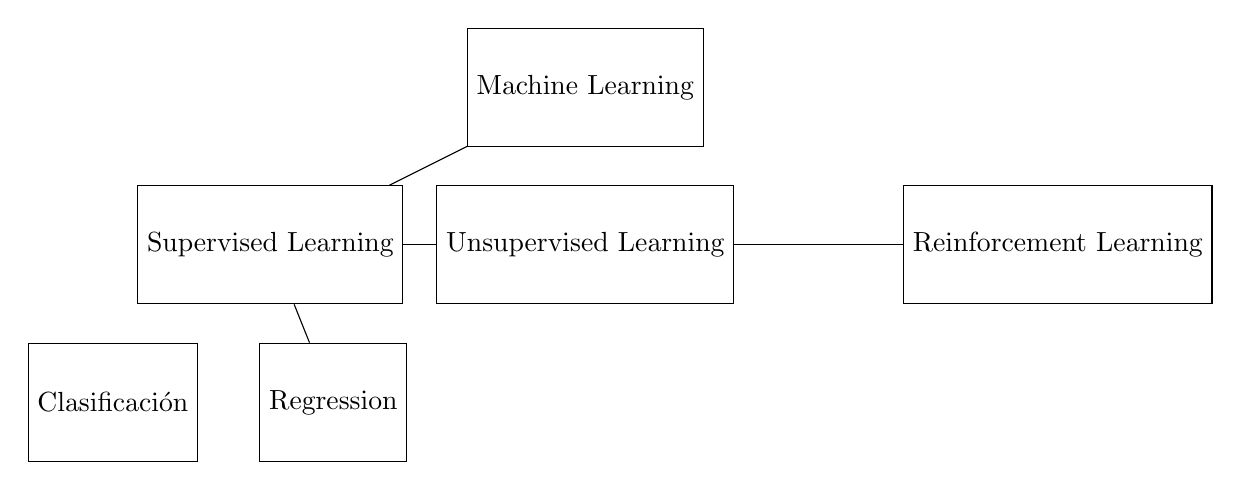
\begin{tikzpicture}[every node/.style={draw, minimum size=1.5cm}]
    % Nodos
    \node (A) at (0,0) {Machine Learning};
    \node (B) at (-4,-2) {Supervised Learning};
    \node (C) at (0,-2) {Unsupervised Learning};
    \node (D) at (6,-2) {Reinforcement Learning};
    \node (E) at (-6,-4) {Clasificaci\'on};
    \node (E) at (-3.2,-4) {Regression};
    
    % Conexiones
    \draw (A) -- (B);
    \draw (B) -- (C);
    \draw (C) -- (D);
    \draw (B) -- (E);


\end{tikzpicture}